\documentclass[14pt,russian]{scrartcl}
\let\counterwithout\relax
\let\counterwithin\relax
\usepackage{lmodern}
\usepackage{float}
\usepackage{xcolor}

\usepackage{extsizes}
\usepackage{subfig}
\usepackage[export]{adjustbox}
\usepackage{tocvsec2} % возможность менять учитываемую глубину разделов в оглавлении
\usepackage[subfigure]{tocloft}

\usepackage{fancyvrb}
\usepackage{ulem,bm,mathrsfs,ifsym} %зачеркивания, особо жирный стиль и RSFS начертание
\usepackage{sectsty} % переопределение стилей подразделов
%%%%%%%%%%%%%%%%%%%%%%%

%%% Поля и разметка страницы %%%
\usepackage{pdflscape}                              % Для включения альбомных страниц
\usepackage{geometry}                               % Для последующего задания полей
\geometry{a4paper,tmargin=2cm,bmargin=2cm,lmargin=3cm,rmargin=1cm} % тоже самое, но лучше

%%% Математические пакеты %%%
\usepackage{amsthm,amsfonts,amsmath,amssymb,amscd}  % Математические дополнения от AMS
\usepackage{mathtools}                              % Добавляет окружение multlined
\usepackage[perpage]{footmisc}

%%%% Установки для размера шрифта 14 pt %%%%
%% Формирование переменных и констант для сравнения (один раз для всех подключаемых файлов)%%
%% должно располагаться до вызова пакета fontspec или polyglossia, потому что они сбивают его работу
%\newlength{\curtextsize}
%\newlength{\bigtextsize}
%\setlength{\bigtextsize}{13pt}
\KOMAoptions{fontsize=14pt}

\makeatletter
\def\showfontsize{\f@size{} point}
\makeatother

%\makeatletter
%\show\f@size                                       % неплохо для отслеживания, но вызывает стопорение процесса, если документ компилируется без команды  -interaction=nonstopmode 
%\setlength{\curtextsize}{\f@size pt}
%\makeatother

%шрифт times
\usepackage{tempora}

   %%% Решение проблемы копирования текста в буфер кракозябрами
%    \input glyphtounicode.tex
%    \input glyphtounicode-cmr.tex %from pdfx package
%    \pdfgentounicode=1
    \usepackage{cmap}                               % Улучшенный поиск русских слов в полученном pdf-файле
    \usepackage[T2A]{fontenc}                       % Поддержка русских букв
    \usepackage[utf8]{inputenc}                     % Кодировка utf8
    \usepackage[english, main=russian]{babel}            % Языки: русский, английский
%   \IfFileExists{pscyr.sty}{\usepackage{pscyr}}{}  % Красивые русские шрифты
%\renewcommand{\rmdefault}{ftm}
%%% Оформление абзацев %%%
\usepackage{indentfirst}                            % Красная строка
%\usepackage{eskdpz}

%%% Таблицы %%%
\usepackage{longtable}                              % Длинные таблицы
\usepackage{multirow,makecell,array}                % Улучшенное форматирование таблиц
\usepackage{booktabs}                               % Возможность оформления таблиц в классическом книжном стиле (при правильном использовании не противоречит ГОСТ)

%%% Общее форматирование
\usepackage{soulutf8}                               % Поддержка переносоустойчивых подчёркиваний и зачёркиваний
\usepackage{icomma}                                 % Запятая в десятичных дробях



%%% Изображения %%%
\usepackage{graphicx}                               % Подключаем пакет работы с графикой
\usepackage{wrapfig}

%%% Списки %%%
\usepackage{enumitem}

%%% Подписи %%%
\usepackage{caption}                                % Для управления подписями (рисунков и таблиц) % Может управлять номерами рисунков и таблиц с caption %Иногда может управлять заголовками в списках рисунков и таблиц
%% Использование:
%\begin{table}[h!]\ContinuedFloat - чтобы не переключать счетчик
%\captionsetup{labelformat=continued}% должен стоять до самого caption
%\caption{}
% либо ручками \caption*{Продолжение таблицы~\ref{...}.} :)

%%% Интервалы %%%

%%% Счётчики %%%
\usepackage[figure,table,section]{totalcount}               % Счётчик рисунков и таблиц
\DeclareTotalCounter{lstlisting}
\usepackage{totcount}                               % Пакет создания счётчиков на основе последнего номера подсчитываемого элемента (может требовать дважды компилировать документ)
\usepackage{totpages}                               % Счётчик страниц, совместимый с hyperref (ссылается на номер последней страницы). Желательно ставить последним пакетом в преамбуле

%%% Продвинутое управление групповыми ссылками (пока только формулами) %%%
%% Кодировки и шрифты %%%

%   \newfontfamily{\cyrillicfont}{Times New Roman}
%   \newfontfamily{\cyrillicfonttt}{CMU Typewriter Text}
	%\setmainfont{Times New Roman}
	%\newfontfamily\cyrillicfont{Times New Roman}
	%\setsansfont{Times New Roman}                    %% задаёт шрифт без засечек
%	\setmonofont{Liberation Mono}               %% задаёт моноширинный шрифт
 %   \IfFileExists{pscyr.sty}{\renewcommand{\rmdefault}{ftm}}{}
%%% Интервалы %%%
%linespread-реализация ближе к реализации полуторного интервала в ворде.
%setspace реализация заточена под шрифты 10, 11, 12pt, под остальные кегли хуже, но всё же ближе к типографской классике. 
\linespread{1.3}                    % Полуторный интервал (ГОСТ Р 7.0.11-2011, 5.3.6)
%\renewcommand{\@biblabel}[1]{#1}

%%% Гиперссылки %%%
\usepackage{hyperref}

%%% Выравнивание и переносы %%%
\sloppy                             % Избавляемся от переполнений
\clubpenalty=10000                  % Запрещаем разрыв страницы после первой строки абзаца
\widowpenalty=10000                 % Запрещаем разрыв страницы после последней строки абзаца

\makeatletter % малые заглавные, small caps shape
\let\@@scshape=\scshape
\renewcommand{\scshape}{%
  \ifnum\strcmp{\f@series}{bx}=\z@
    \usefont{T1}{cmr}{bx}{sc}%
  \else
    \ifnum\strcmp{\f@shape}{it}=\z@
      \fontshape{scsl}\selectfont
    \else
      \@@scshape
    \fi
  \fi}
\makeatother

%%% Подписи %%%
%\captionsetup{%
%singlelinecheck=off,                % Многострочные подписи, например у таблиц
%skip=2pt,                           % Вертикальная отбивка между подписью и содержимым рисунка или таблицы определяется ключом
%justification=centering,            % Центрирование подписей, заданных командой \caption
%}
%%%        Подключение пакетов                 %%%
\usepackage{ifthen}                 % добавляет ifthenelse
%%% Инициализирование переменных, не трогать!  %%%
\newcounter{intvl}
\newcounter{otstup}
\newcounter{contnumeq}
\newcounter{contnumfig}
\newcounter{contnumtab}
\newcounter{pgnum}
\newcounter{bibliosel}
\newcounter{chapstyle}
\newcounter{headingdelim}
\newcounter{headingalign}
\newcounter{headingsize}
\newcounter{tabcap}
\newcounter{tablaba}
\newcounter{tabtita}
%%%%%%%%%%%%%%%%%%%%%%%%%%%%%%%%%%%%%%%%%%%%%%%%%%

%%% Область упрощённого управления оформлением %%%

%% Интервал между заголовками и между заголовком и текстом
% Заголовки отделяют от текста сверху и снизу тремя интервалами (ГОСТ Р 7.0.11-2011, 5.3.5)
\setcounter{intvl}{3}               % Коэффициент кратности к размеру шрифта

%% Отступы у заголовков в тексте
\setcounter{otstup}{0}              % 0 --- без отступа; 1 --- абзацный отступ

%% Нумерация формул, таблиц и рисунков
\setcounter{contnumeq}{1}           % Нумерация формул: 0 --- пораздельно (во введении подряд, без номера раздела); 1 --- сквозная нумерация по всей диссертации
\setcounter{contnumfig}{1}          % Нумерация рисунков: 0 --- пораздельно (во введении подряд, без номера раздела); 1 --- сквозная нумерация по всей диссертации
\setcounter{contnumtab}{1}          % Нумерация таблиц: 0 --- пораздельно (во введении подряд, без номера раздела); 1 --- сквозная нумерация по всей диссертации

%% Оглавление
\setcounter{pgnum}{0}               % 0 --- номера страниц никак не обозначены; 1 --- Стр. над номерами страниц (дважды компилировать после изменения)

%% Библиография
\setcounter{bibliosel}{1}           % 0 --- встроенная реализация с загрузкой файла через движок bibtex8; 1 --- реализация пакетом biblatex через движок biber

%% Текст и форматирование заголовков
\setcounter{chapstyle}{1}           % 0 --- разделы только под номером; 1 --- разделы с названием "Глава" перед номером
\setcounter{headingdelim}{1}        % 0 --- номер отделен пропуском в 1em или \quad; 1 --- номера разделов и приложений отделены точкой с пробелом, подразделы пропуском без точки; 2 --- номера разделов, подразделов и приложений отделены точкой с пробелом.

%% Выравнивание заголовков в тексте
\setcounter{headingalign}{0}        % 0 --- по центру; 1 --- по левому краю

%% Размеры заголовков в тексте
\setcounter{headingsize}{0}         % 0 --- по ГОСТ, все всегда 14 пт; 1 --- пропорционально изменяющийся размер в зависимости от базового шрифта

%% Подпись таблиц
\setcounter{tabcap}{0}              % 0 --- по ГОСТ, номер таблицы и название разделены тире, выровнены по левому краю, при необходимости на нескольких строках; 1 --- подпись таблицы не по ГОСТ, на двух и более строках, дальнейшие настройки: 
%Выравнивание первой строки, с подписью и номером
\setcounter{tablaba}{2}             % 0 --- по левому краю; 1 --- по центру; 2 --- по правому краю
%Выравнивание строк с самим названием таблицы
\setcounter{tabtita}{1}             % 0 --- по левому краю; 1 --- по центру; 2 --- по правому краю

%%% Рисунки %%%
\DeclareCaptionLabelSeparator*{emdash}{~--- }             % (ГОСТ 2.105, 4.3.1)
\captionsetup[figure]{labelsep=emdash,font=onehalfspacing,position=bottom}

%%% Таблицы %%%
\ifthenelse{\equal{\thetabcap}{0}}{%
    \newcommand{\tabcapalign}{\raggedright}  % по левому краю страницы или аналога parbox
}

\ifthenelse{\equal{\thetablaba}{0} \AND \equal{\thetabcap}{1}}{%
    \newcommand{\tabcapalign}{\raggedright}  % по левому краю страницы или аналога parbox
}

\ifthenelse{\equal{\thetablaba}{1} \AND \equal{\thetabcap}{1}}{%
    \newcommand{\tabcapalign}{\centering}    % по центру страницы или аналога parbox
}

\ifthenelse{\equal{\thetablaba}{2} \AND \equal{\thetabcap}{1}}{%
    \newcommand{\tabcapalign}{\raggedleft}   % по правому краю страницы или аналога parbox
}

\ifthenelse{\equal{\thetabtita}{0} \AND \equal{\thetabcap}{1}}{%
    \newcommand{\tabtitalign}{\raggedright}  % по левому краю страницы или аналога parbox
}

\ifthenelse{\equal{\thetabtita}{1} \AND \equal{\thetabcap}{1}}{%
    \newcommand{\tabtitalign}{\centering}    % по центру страницы или аналога parbox
}

\ifthenelse{\equal{\thetabtita}{2} \AND \equal{\thetabcap}{1}}{%
    \newcommand{\tabtitalign}{\raggedleft}   % по правому краю страницы или аналога parbox
}

\DeclareCaptionFormat{tablenocaption}{\tabcapalign #1\strut}        % Наименование таблицы отсутствует
\ifthenelse{\equal{\thetabcap}{0}}{%
    \DeclareCaptionFormat{tablecaption}{\tabcapalign #1#2#3}
    \captionsetup[table]{labelsep=emdash}                       % тире как разделитель идентификатора с номером от наименования
}{%
    \DeclareCaptionFormat{tablecaption}{\tabcapalign #1#2\par%  % Идентификатор таблицы на отдельной строке
        \tabtitalign{#3}}                                       % Наименование таблицы строкой ниже
    \captionsetup[table]{labelsep=space}                        % пробельный разделитель идентификатора с номером от наименования
}
\captionsetup[table]{format=tablecaption,singlelinecheck=off,font=onehalfspacing,position=top,skip=-5pt}  % многострочные наименования и прочее
\DeclareCaptionLabelFormat{continued}{Продолжение таблицы~#2}
\setlength{\belowcaptionskip}{.2cm}
\setlength{\intextsep}{0ex}

%%% Подписи подрисунков %%%
\renewcommand{\thesubfigure}{\asbuk{subfigure}}           % Буквенные номера подрисунков
\captionsetup[subfigure]{font={normalsize},               % Шрифт подписи названий подрисунков (не отличается от основного)
    labelformat=brace,                                    % Формат обозначения подрисунка
    justification=centering,                              % Выключка подписей (форматирование), один из вариантов            
}
%\DeclareCaptionFont{font12pt}{\fontsize{12pt}{13pt}\selectfont} % объявляем шрифт 12pt для использования в подписях, тут же надо интерлиньяж объявлять, если не наследуется
%\captionsetup[subfigure]{font={font12pt}}                 % Шрифт подписи названий подрисунков (всегда 12pt)

%%% Настройки гиперссылок %%%

\definecolor{linkcolor}{rgb}{0.0,0,0}
\definecolor{citecolor}{rgb}{0,0.0,0}
\definecolor{urlcolor}{rgb}{0,0,0}

\hypersetup{
    linktocpage=true,           % ссылки с номера страницы в оглавлении, списке таблиц и списке рисунков
%    linktoc=all,                % both the section and page part are links
%    pdfpagelabels=false,        % set PDF page labels (true|false)
    plainpages=true,           % Forces page anchors to be named by the Arabic form  of the page number, rather than the formatted form
    colorlinks,                 % ссылки отображаются раскрашенным текстом, а не раскрашенным прямоугольником, вокруг текста
    linkcolor={linkcolor},      % цвет ссылок типа ref, eqref и подобных
    citecolor={citecolor},      % цвет ссылок-цитат
    urlcolor={urlcolor},        % цвет гиперссылок
    pdflang={ru},
}
\urlstyle{same}
%%% Шаблон %%%
%\DeclareRobustCommand{\todo}{\textcolor{red}}       % решаем проблему превращения названия цвета в результате \MakeUppercase, http://tex.stackexchange.com/a/187930/79756 , \DeclareRobustCommand protects \todo from expanding inside \MakeUppercase
\setlength{\parindent}{2.5em}                       % Абзацный отступ. Должен быть одинаковым по всему тексту и равен пяти знакам (ГОСТ Р 7.0.11-2011, 5.3.7).

%%% Списки %%%
% Используем дефис для ненумерованных списков (ГОСТ 2.105-95, 4.1.7)
%\renewcommand{\labelitemi}{\normalfont\bfseries~{---}} 
\renewcommand{\labelitemi}{\bfseries~{---}} 
\setlist{nosep,%                                    % Единый стиль для всех списков (пакет enumitem), без дополнительных интервалов.
    labelindent=\parindent,leftmargin=*%            % Каждый пункт, подпункт и перечисление записывают с абзацного отступа (ГОСТ 2.105-95, 4.1.8)
}
%%%%%%%%%%%%%%%%%%%%%%
%\usepackage{xltxtra} % load xunicode

\usepackage{ragged2e}
\usepackage[explicit]{titlesec}
\usepackage{placeins}
\usepackage{xparse}

\usepackage{listingsutf8}
\usepackage{url} %пакеты расширений
\usepackage{algorithm, algorithmicx}
\usepackage[noend]{algpseudocode}
\usepackage{blkarray}
\usepackage{chngcntr}
\usepackage{tabularx}
\newcommand*\template[1]{\text{<}#1\text{>}}

  
\titleformat{name=\section,numberless}[block]{\normalfont\Large\centering}{}{0em}{#1}
\titleformat{\section}[block]{\normalfont\Large\bfseries\raggedright}{}{0em}{\thesection\hspace{0.25em}#1}
\titleformat{\subsection}[block]{\normalfont\Large\bfseries\raggedright}{}{0em}{\thesubsection\hspace{0.25em}#1}
\titleformat{\subsubsection}[block]{\normalfont\large\bfseries\raggedright}{}{0em}{\thesubsubsection\hspace{0.25em}#1}

\let\Algorithm\algorithm
\renewcommand\algorithm[1][]{\Algorithm[#1]\setstretch{1.5}}

\usepackage{pifont}
\usepackage{calc}
\usepackage{suffix}
\usepackage{csquotes}
\DeclareQuoteStyle{russian}
    {\guillemotleft}{\guillemotright}[0.025em]
    {\quotedblbase}{\textquotedblleft}
\ExecuteQuoteOptions{style=russian}
\newcommand{\enq}[1]{\enquote{#1}}  
\newcommand{\eng}[1]{\begin{english}#1\end{english}}
% Подчиненные счетчики в окружениях http://old.kpfu.ru/journals/izv_vuz/arch/sample1251.tex
\newcounter{cTheorem} 
\newcounter{cDefinition}
\newcounter{cConsequent}
\newcounter{cExample}
\newcounter{cLemma}
\newcounter{cConjecture}
\newtheorem{Theorem}{Теорема}[cTheorem]
\newtheorem{Definition}{Определение}[cDefinition]
\newtheorem{Consequent}{Следствие}[cConsequent]
\newtheorem{Example}{Пример}[cExample]
\newtheorem{Lemma}{Лемма}[cLemma]
\newtheorem{Conjecture}{Гипотеза}[cConjecture]

\renewcommand{\theTheorem}{\arabic{Theorem}}
\renewcommand{\theDefinition}{\arabic{Definition}}
\renewcommand{\theConsequent}{\arabic{Consequent}}
\renewcommand{\theExample}{\arabic{Example}}
\renewcommand{\theLemma}{\arabic{Lemma}}
\renewcommand{\theConjecture}{\arabic{Conjecture}}
%\makeatletter
\NewDocumentCommand{\Newline}{}{\text{\\}}
\newcommand{\sequence}[2]{\ensuremath \left(#1,\ \dots,\ #2\right)}

\definecolor{mygreen}{rgb}{0,0.6,0}
\definecolor{mygray}{rgb}{0.5,0.5,0.5}
\definecolor{mymauve}{rgb}{0.58,0,0.82}
\renewcommand{\listalgorithmname}{Список алгоритмов}
\floatname{algorithm}{Листинг}
\renewcommand{\lstlistingname}{Листинг}
\renewcommand{\thealgorithm}{\arabic{algorithm}}

\newcommand{\refAlgo}[1]{(листинг \ref{#1})}
\newcommand{\refImage}[1]{(рисунок \ref{#1})}

\renewcommand{\theenumi}{\arabic{enumi}.}% Меняем везде перечисления на цифра.цифра	
\renewcommand{\labelenumi}{\arabic{enumi}.}% Меняем везде перечисления на цифра.цифра
\renewcommand{\theenumii}{\arabic{enumii}}% Меняем везде перечисления на цифра.цифра
\renewcommand{\labelenumii}{(\arabic{enumii})}% Меняем везде перечисления на цифра.цифра
\renewcommand{\theenumiii}{\roman{enumiii}}% Меняем везде перечисления на цифра.цифра
\renewcommand{\labelenumiii}{(\roman{enumiii})}% Меняем везде перечисления на цифра.цифра
%\newfontfamily\AnkaCoder[Path=src/fonts/]{AnkaCoder-r.ttf}
\renewcommand{\labelitemi}{---}
\renewcommand{\labelitemii}{---}

%\usepackage{courier}

\graphicspath{ {./img/} }

\lstdefinelanguage{Refal}{
  alsodigit = {.,<,>},
  morekeywords = [1]{$ENTRY},
  morekeywords = [2]{Go, Put, Get, Open, Close, Arg, Add, Sub, Mul, Div, Symb, Explode, Implode},
  %keyword4
  morekeywords = [3]{<,>},
  %keyword5
  morekeywords = [4]{e.,t.,s.},
  sensitive = true,
  morecomment = [l]{*},
  morecomment = [s]{/*}{*/},
  commentstyle = \color{mygreen},
  morestring = [b]",
  morestring = [b]',
  stringstyle = \color{purple}
}

\makeatletter
\def\p@subsection{}
\def\p@subsubsection{\thesection\,\thesubsection\,}
\makeatother
\newcommand{\prog}[1]{{\ttfamily\small#1}}
\lstset{ %
  backgroundcolor=\color{white},   % choose the background color; you must add \usepackage{color} or \usepackage{xcolor}
  basicstyle=\ttfamily\footnotesize, 
  %basicstyle=\footnotesize\AnkaCoder,        % the size of the fonts that are used for the code
  breakatwhitespace=false,         % sets if automatic breaks shoulbd only happen at whitespace
  breaklines=true,                 % sets automatic line breaking
  captionpos=top,                    % sets the caption-position to bottom
  commentstyle=\color{mygreen},    % comment style
  deletekeywords={...},            % if you want to delete keywords from the given language
  escapeinside={\%*}{*)},          % if you want to add LaTeX within your code
  extendedchars=true,              % lets you use non-ASCII characters; for 8-bits encodings only, does not work with UTF-8
  inputencoding=utf8,
  frame=single,                    % adds a frame around the code
  keepspaces=true,                 % keeps spaces in text, useful for keeping indentation of code (possibly needs columns=flexible)
  keywordstyle=\bf,       % keyword style
  language=Refal,                    % the language of the code
  morekeywords={<,>,$ENTRY,Go,Arg, Open, Close, e., s., t., Get, Put}, 
  							       % if you want to add more keywords to the set
  numbers=left,                    % where to put the line-numbers; possible values are (none, left, right)
  numbersep=5pt,                   % how far the line-numbers are from the code
  xleftmargin=25pt,
  xrightmargin=25pt,
  numberstyle=\small\color{black}, % the style that is used for the line-numbers
  rulecolor=\color{black},         % if not set, the frame-color may be changed on line-breaks within not-black text (e.g. comments (green here))
  showspaces=false,                % show spaces everywhere adding particular underscores; it overrides 'showstringspaces'
  showstringspaces=false,          % underline spaces within strings only
  showtabs=false,                  % show tabs within strings adding particular underscores
  stepnumber=1,                    % the step between two line-numbers. If it's 1, each line will be numbered
  stringstyle=\color{mymauve},     % string literal style
  tabsize=8,                       % sets default tabsize to 8 spaces
  title=\lstname                   % show the filename of files included with \lstinputlisting; also try caption instead of title
}
\newcommand{\anonsection}[1]{\cleardoublepage
\phantomsection
\addcontentsline{toc}{section}{\protect\numberline{}#1}
\section*{#1}\vspace*{2.5ex} % По госту положены 3 пустые строки после заголовка ненумеруемого раздела
}
\newcommand{\sectionbreak}{\clearpage}
\renewcommand{\sectionfont}{\normalsize} % Сбиваем стиль оглавления в стандартный
\renewcommand{\cftsecleader}{\cftdotfill{\cftdotsep}} % Точки в оглавлении напротив разделов

\renewcommand{\cftsecfont}{\normalfont\large} % Переключение на times в содержании
\renewcommand{\cftsubsecfont}{\normalfont\large} % Переключение на times в содержании

\usepackage{caption} 
%\captionsetup[table]{justification=raggedleft} 
%\captionsetup[figure]{justification=centering,labelsep=endash}
\usepackage{amsmath}    % \bar    (матрицы и проч. ...)
\usepackage{amsfonts}   % \mathbb (символ для множества действительных чисел и проч. ...)
\usepackage{mathtools}  % \abs, \norm
    \DeclarePairedDelimiter\abs{\lvert}{\rvert} % операция модуля
    \DeclarePairedDelimiter\norm{\lVert}{\rVert} % операция нормы
\DeclareTextCommandDefault{\textvisiblespace}{%
  \mbox{\kern.06em\vrule \@height.3ex}%
  \vbox{\hrule \@width.3em}%
  \hbox{\vrule \@height.3ex}}    
\newsavebox{\spacebox}
\begin{lrbox}{\spacebox}
\verb*! !
\end{lrbox}
\newcommand{\aspace}{\usebox{\spacebox}}

\title{Lab 01 report}
\author{Sergey}

\date{\today}

\begin{document}
\thispagestyle{empty}

\noindent \begin{minipage}{0.15\textwidth}
	
\includegraphics[width=\linewidth]{b_logo}
\end{minipage}
\noindent\begin{minipage}{0.85\textwidth}\centering
	\textbf{Министерство науки и высшего образования Российской Федерации}\\
	\textbf{Федеральное государственное бюджетное образовательное учреждение высшего образования}\\
	\textbf{«Московский государственный технический университет имени Н. Э.~Баумана}\\
	\textbf{(национальный исследовательский университет)»}\\
	\textbf{(МГТУ им. Н. Э.~Баумана)}
\end{minipage}

\noindent\rule{16cm}{3pt}
\newline\newline
\noindent ФАКУЛЬТЕТ $\underline{\text{«Информатика и системы управления»}}$ \newline\newline
\noindent КАФЕДРА $\underline{\text{«Программное обеспечение ЭВМ и информационные технологии»}}$\newline


\begin{center}
	\noindent\begin{minipage}{1.3\textwidth}\centering
	\Large\textbf{   ~~~ Лабораторная работа №1}\newline
	\textbf{по дисциплине "Анализ Алгоритмов"}\newline\newline\newline
	\end{minipage}
\end{center}

\noindent\textbf{Тема} $\underline{\text{Расстояние Левенштейна}}$\newline\newline
\noindent\textbf{Студент} $\underline{\text{Сабуров С. М.}}$\newline\newline
\noindent\textbf{Группа} $\underline{\text{ИУ7-53Б}}$\newline\newline
\noindent\textbf{Преподаватель} $\underline{\text{Волкова Л. Л.}}$\newline

\begin{center}
	\mbox{}
	\vfill
	Москва
\end{center}

\begin{center}
	\the\year ~г.
\end{center}
\clearpage


\renewcommand\contentsname{\hfill{\normalfont{СОДЕРЖАНИЕ}}\hfill}  %Оглавление
\tableofcontents
\newpage

\anonsection{Введение}
	
\textbf{Расстояние Левенштейна} - минимальное количество операций вставки одного символа, удаления одного символа и замены одного символа на другой, необходимых для превращения одной строки в другую.

Расстояние Левенштейна применяется в теории информации и компьютерной лингвистике для следущего:

\begin{itemize}
	\item исправления ошибок в слове;
	\item сравнения текстовых файлов утилитой diff;
	\item в биоинформатике для сравнения генов, хромосом и белков.
\end{itemize}

\textit{Цель данной лабораторной работы:} реализация и анализ алгоритмов нахождения расстояние Левенштейна и Дамерау-Левенштейна.\\

Для достижения поставленной цели необходимо выполнить следующие задачи:
\begin{enumerate}
	\item Изучение алгоритмов Левенштейна и Дамерау-Левенштейна нахождения расстояния между строками.
	\item Применение метода динамического программирования для матричной реализации указанных алгоритмов.
	\item Получение практических навыков реализации указанных алгоритмов: двух алгоритмов в матричной версии и одного из алгоритмов в рекурсивной версии.
	\item Сравнительный анализ линейной и рекурсивной реализаций выбранного алгоритма определения расстояния между строками по затрачиваемым ресурсам (времени и памяти).
	\item Экспериментальное подтверждение различий во временнóй эффективности рекурсивной и
	      нерекурсивной реализаций выбранного алгоритма определения расстояния между строками при
	      помощи разработанного программного обеспечения на материале замеров процессорного времени
	      выполнения реализации на варьирующихся длинах строк.
	\item Описание и обоснование полученных результатов в отчете о выполненной лабораторной
	      работе, выполненного как расчётно-пояснительная записка к работе. 
\end{enumerate}

\section{Аналитическая часть}
Расстояние Левенштейна [2] между двумя строками ~--~ это минимальное количество операций вставки, удаления и замены, необходимых для превращения одной строки в другую

Цены операций могут зависеть от вида операций (вставка, удаление, замена) и/или от участвующих в ней символов, отражая разную вероятность разных ошибок при вводе текста и т.п. В общем случае

\begin{itemize}
	\item $w(a, b)$ ~--~ цена замены символа $a$ на $b$;
	\item $w(\lambda, b)$ ~--~ цена вставки символа $b$;
	\item $w(a, \lambda)$ ~--~ цена удаления символа $a$.
\end{itemize}

Для решения задачи о редакционном расстоянии необходимо найти последовательность замен, минимизирующую суммарную цену. Расстояние Левенштейна является частным случаем это задачи при

\begin{itemize}
	\item $w(a, a) = 0$;
	\item $w(a, b) = 1$, $a \neq b$;
	\item $w(\lambda, b) = 1$;
	\item $w(a, \lambda) = 1$.
\end{itemize}

\subsection{Расстояние Левенштейна}

Пусть $S_{1}$ и $S_{2}$ — две строки (длиной M и N соответственно) над некоторым алфавитом, тогда расстояние Левенштейна можно подсчитать по следующей рекуррентной формуле:

\begin{displaymath}
	D(i,j) = \left\{ \begin{array}{ll}
	0, & \textrm{$i = 0, j = 0$}\\
	i, & \textrm{$j = 0, i > 0$}\\
	j, & \textrm{$i = 0, j > 0$}\\
	min(\\
	D(i,j-1)+1,\\
	D(i-1, j) +1, &\textrm{$j>0, i>0$}\\
	D(i-1, j-1) + m(S_{1}[i], S_{2}[j])\\
	),
	\end{array} \right.
\end{displaymath}

\noindent
где $m(a,b)$ равна нулю, если $a=b$ и единице в противном случае; $min\{\,a,b,c\}$ возвращает наименьший из аргументов.

\subsection{Расстояние Дамерау-Левенштейна}

Расстояние Дамерау-Левенштейна вычисляется по следующей рекуррентной формуле:
		    
\[ D(i, j) =  \left\{
	\begin{aligned}
		  & 0, &   & i = 0, j = 0 \\
		  & i, &   & i > 0, j = 0 \\
		  & j, &   & i = 0, j > 0 \\		    	
		&min \left\{
		\begin{aligned}
		&D(i, j - 1) + 1,\\
		&D(i - 1, j) + 1,\\
		&D(i - 1, j - 1) + m(S_{1}[i], S_{2}[i]), \\
		&D(i - 2, j - 2) + m(S_{1}[i], S_{2}[i]),\\
	\end{aligned} \right.
	&& 
	\begin{aligned}
		  & , \text{ если } i, j > 0         \\
		  & \text{ и } S_{1}[i] = S_{2}[j - 1]  \\
		  & \text{ и } S_{1}[i - 1] =  S_{2}[j] \\
	\end{aligned} \\ 
	&min \left\{
	\begin{aligned}
		  & D(i, j - 1) + 1,                         \\
		  & D(i - 1, j) + 1,                         \\
		  & D(i - 1, j - 1) + m(S_{1}[i], S_{2}[i]). \\
	\end{aligned} \right.  &&, \text{иначе}
	\end{aligned} \right.
\]	
	    
\subsection{Вывод}

В данном разделе были рассмотрены алгоритмы нахождения расстояния Левенштейна и Дамерау-Левенштейна, который является модификаций первого, учитывающего возможность перестановки соседних символов. 
\begin{itemize}
	\item Входные данные — на вход подаются две строки. Заглавные и прописные буквы считаются разными.
	\item Выходные данные — на выходе имеем целое число.
	\item Ограничения, в рамках которых будет работать программа — Две пустые строки - корректный ввод, программа не должна аварийно завершаться.
	\item Функциональные требования — функции, представленные на листингах 1 - 3 должны вычислять расстояние Левенштейна, принимая на вход 2 строки и длины этих строк и возвращая целое число. Функция представленная на листинге 4 должна вычислять расстояние Дамерау - Левенштейна, принимая на вход 2 строки и длины этих строк и возвращая целое число.
\end{itemize}
		
\section{Конструкторская часть}

В данном разделе будут приведены схемы алгоритмов

		
\subsection{Схемы алгоритмов}
На рис. \ref{fig:rec_lev}-\ref{fig:iter_dam_lev2}  показаны схемы рассматриваемых алгоритмов.
\begin{figure}[h]
	\centering
	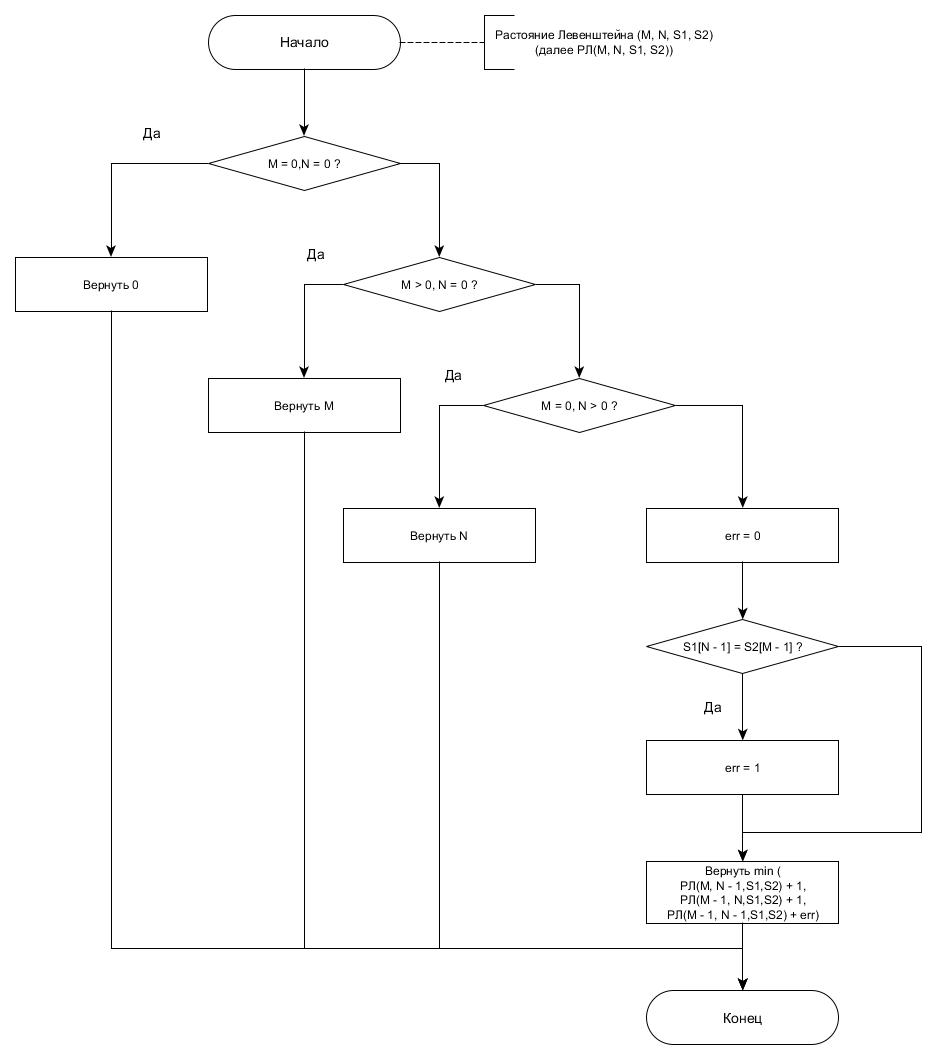
\includegraphics[scale=0.5]{rec_lev.jpg}
	\caption{Схема рекурсивного алгоритма нахождения расстояния Левенштейна}
	\label{fig:rec_lev}
\end{figure}

\begin{figure}[h]
	\centering
	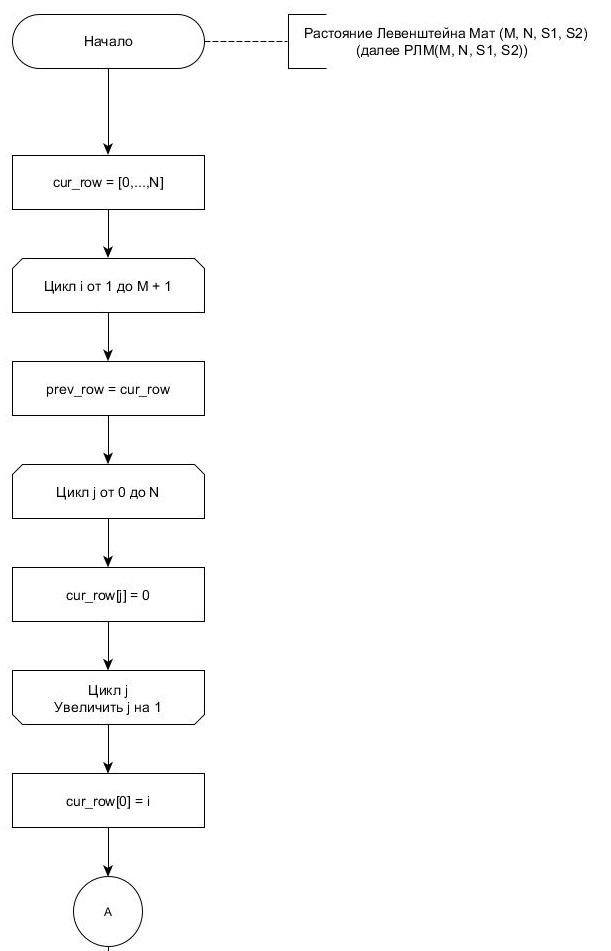
\includegraphics[scale=0.9]{matr_lev11.jpg}
	\caption{Схема матричного алгоритма нахождения расстояния Левенштейна. Часть 1}
	\label{fig:iter_lev}
\end{figure}

\begin{figure}[h]
	\centering
	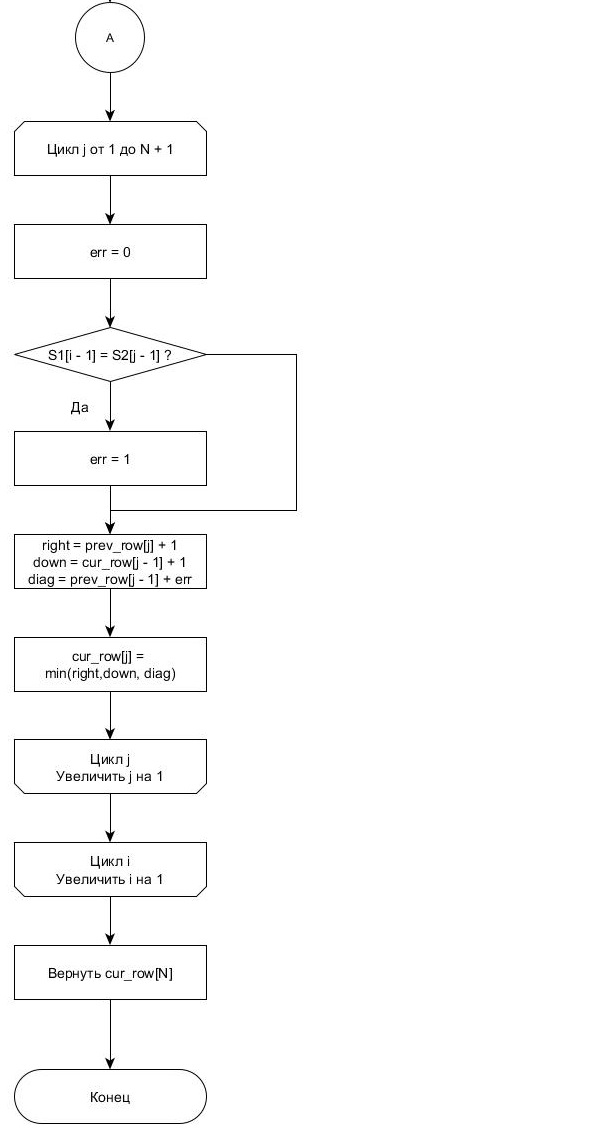
\includegraphics[scale=0.9]{matr_lev12.jpg}
	\caption{Схема матричного алгоритма нахождения расстояния Левенштейна. Часть 2}
	\label{fig:iter_lev2}
\end{figure}



\begin{figure}[h]
	\centering
	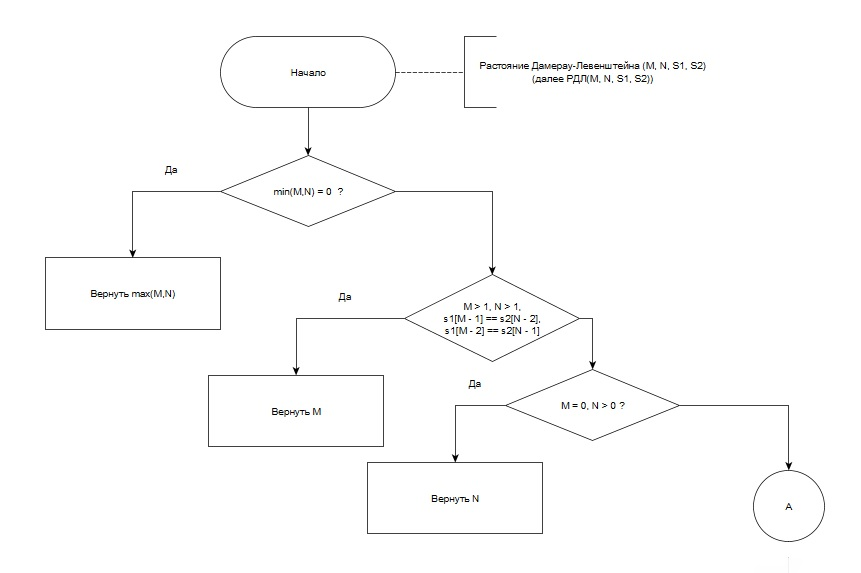
\includegraphics[scale=0.85]{damer-lev_rec1.jpg}
	\caption{Схема рекурсивного алгоритма нахождения расстояния Дамерау-Левенштейна. Часть 1}
	\label{fig:rec_dam_lev1}
\end{figure}

\begin{figure}[h]
	\centering
	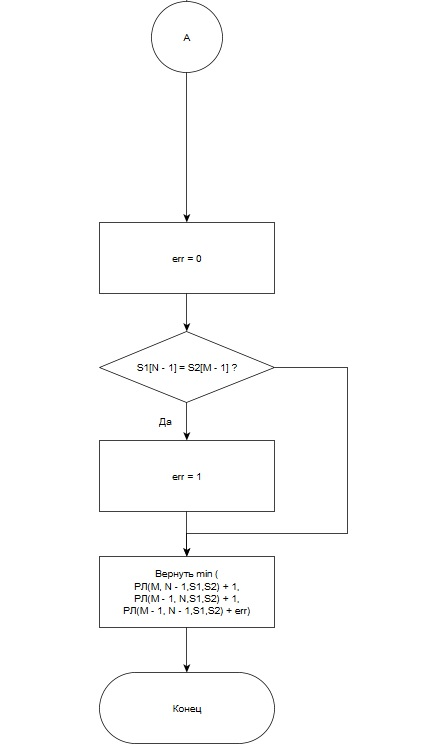
\includegraphics[scale=0.85]{damer-lev_rec2.jpg}
	\caption{Схема рекурсивного алгоритма нахождения расстояния Дамерау-Левенштейна. Часть 2}
	\label{fig:rec_dam_lev2}
\end{figure}

\begin{figure}[h]
	\centering
	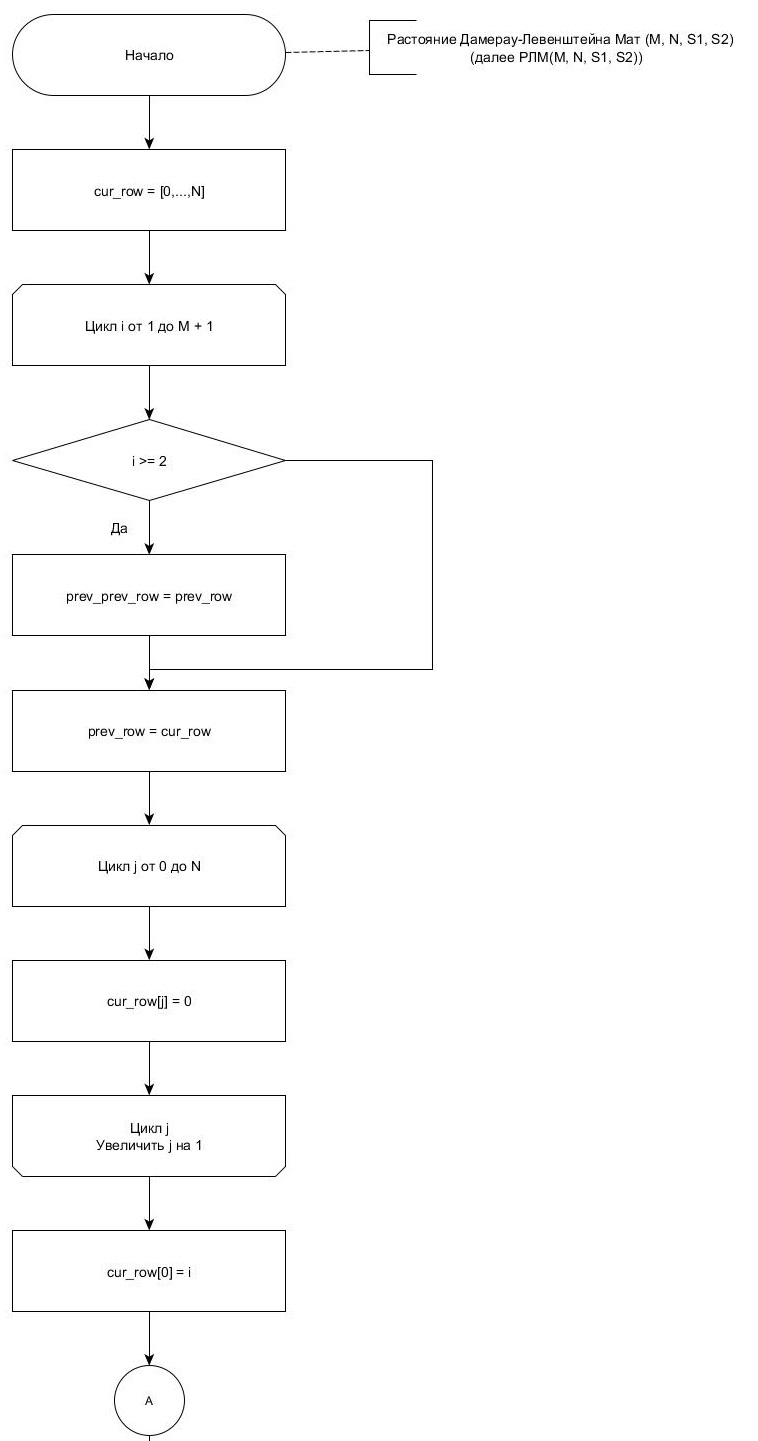
\includegraphics[width=0.7\linewidth]{damer-lev_matr_11.jpg}
	\caption{Схема матричного алгоритма нахождения расстояния Дамерау-Левенштейна. Часть 1}
	\label{fig:iter_dam_lev1}
\end{figure}

\begin{figure}[h]
	\centering
	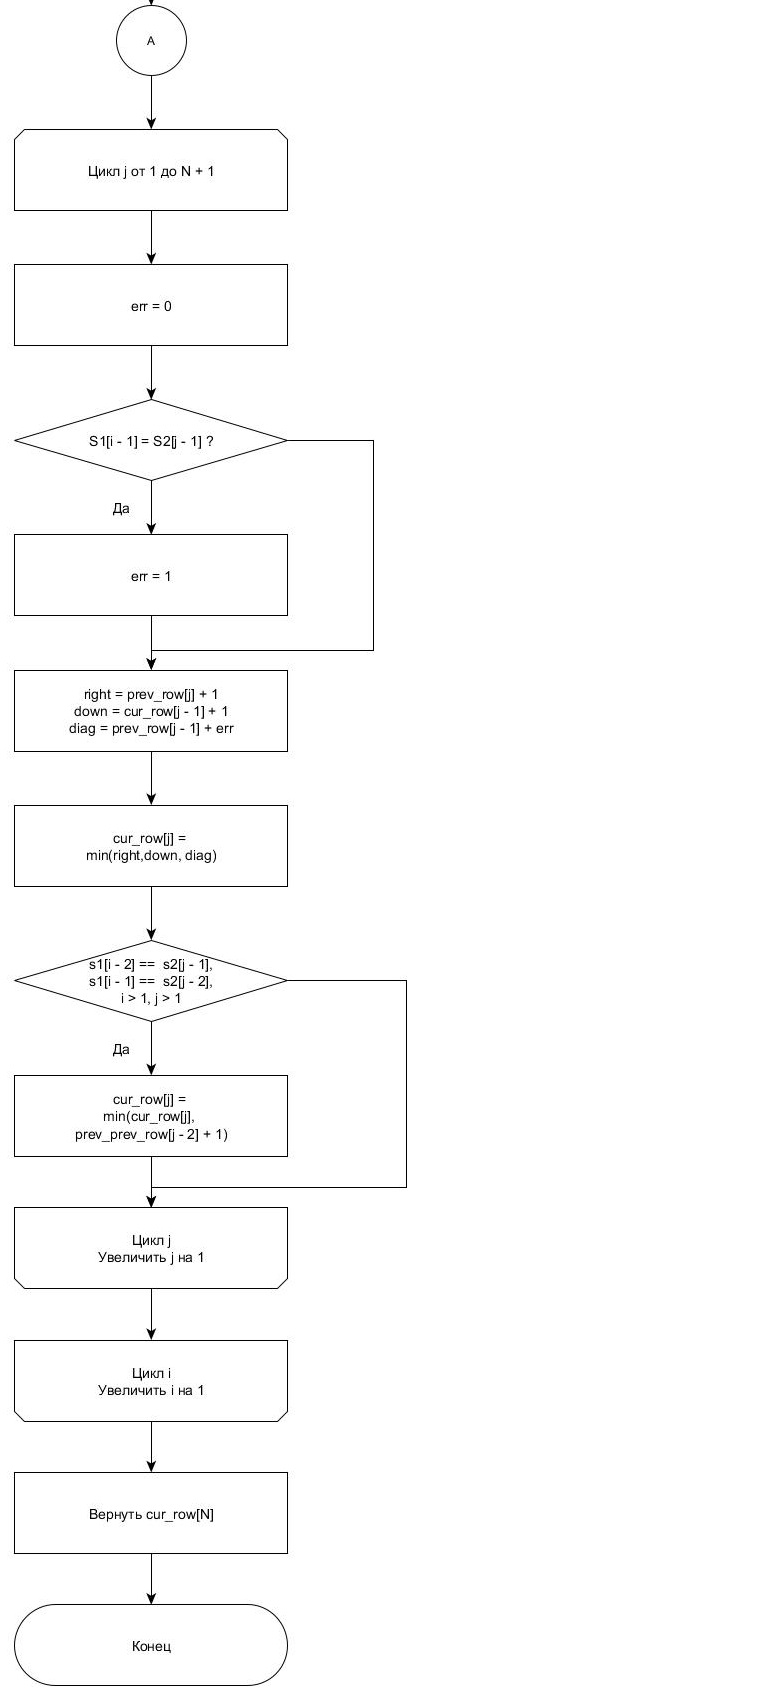
\includegraphics[width=0.65\linewidth]{damer-lev_matr_12.jpg}
	\caption{Схема матричного алгоритма нахождения расстояния Дамерау-Левенштейна. Часть 2}
	\label{fig:iter_dam_lev2}
\end{figure}

\subsection{Описание структур данных}
В алгоритмах, где подразумевается работа с матрицей, используются 2 массива, содержащий последовательно идущие строки матрицы. Такой выбор был сделан из соображений экономии памяти.

\subsection{Способы тестирования и классы эквивалентности}
Была выбрана методика тестирования черным ящиком. 
Классы эквивалентности:
\begin{itemize}
	\item Одинаковые строки.
	\item Строки, отличающиеся в один символ .
	\item Пустые строки.
	\item Строки, полностью отличающиеся по символьному содержанию .
\end{itemize}

\subsection{Использование памяти}

	\par
	Алгоритмы Левенштейна и Дамерау-Левенштейна не отличаются по использованию памяти, соответственно достаточно рассмотреть рекурсивный и матричный реализации этих алгоритмов.

	\par
	Максимальная глубина стека вызовов при рекурсивной реализации равна сумме длин входящих строк, а на каждый вызов функции требуется еще 5 дополнительных переменных типа \textit{usize}, соответственно, максимальный расход памяти

	\begin{equation}
		(Size(S_{1}) + Size(S_{2}) \cdot (2 \cdot Size(\text{string}) + 5 \cdot Size(\text{usize})))
	\end{equation}
	
	\noindent
	где Size - функция, возвращающая размер аргумента; string - строковый тип, usize - целочисленный, беззнаковый тип.

	\par
	Использование памяти при итеративной реализации теоритически равно

	\begin{equation}
		\label{eq:mem_req}
		(Size(S_{1} + 1) \cdot Size(S_{2} + 1)) \cdot Size(usize) + 2 \cdot Size(string)
	\end{equation}

	\par
	Использование памяти рекурсивной реализации алгоритма Левенштейна с кэшем теоритически равно

	\begin{multline}
		\label{eq:mem_iter}
		(Size(S_{1}) + Size(S_{2}) \cdot (2 \cdot Size(string) +\\+ 5 \cdot Size(usize)) + (Size(S_{1} + 1) \cdot Size(S_{2} + 1)) \cdot Size(usize))
	\end{multline}
	\subsection{Вывод}

	\par
	Рекурсивный алгоритм Левенштейна работает на порядок дольше итеративных реализаций, время его работы увеличивается в геометрической прогрессии. На словах длиной 9 символов, матричная реализация превосходит рекурсивную в 4800 раз. Рекурсивные алгоритмы Левенштейна и Дамерау - Левенштейна сопостовимы по времени. Однако, использование кэша значительно ускоряет рекурсивный алгоритм, но он все еще не превосходит матричную реализацию.

	Из формул \ref{eq:mem_req}-\ref{eq:mem_iter} можно сделать вывод, что рекурсивные алгоритмы потребляют больше памяти, чем матричные, при одинаковых длин строк.
\section{Технологическая часть}

В данном разделе приведены листинги реализаций алгоритмов, тестирование и выбор языка программирования.


\subsection{Выбор языка программирования}
Для реализации программ я выбрал язык программирования Python [1], так как этот язык предоставляет как низкоуровневые интерфейсы, так и высокоуровневые. Также он является безопасным языком. Среда разработки IDLE. Также данный язык был выбран потому, что в нем присутствует инструментарий для замера процессорного времени и тестирования.

\subsection{Листинги реализации алгоритма}
В листингах 3.1 - 3.4 приведена реализация алгоритмов нахождения расстояния Левенштейна и Дамерау-Левенштейна.

\begin{lstlisting}[label=some-code,caption=Функция нахождения расстояния Левенштейна рекурсивно,language=Python]
def lev_rec(M,N, s1,s2):
    if (M == 0 and N == 0):
        return 0
    elif (M > 0 and N == 0):
        return M
    elif (M == 0 and N > 0):
        return N
    else:
        return min(lev_rec(M, N - 1,s1,s2) + 1,\
                   lev_rec(M - 1, N,s1,s2) + 1,\
                   lev_rec(M - 1, N - 1,s1,s2) + bool(ord(s1[M - 1]) - ord(s2[N - 1])))
\end{lstlisting}
\clearpage

\begin{lstlisting}[label=some-code,caption=Функция нахождения расстояние Левенштейна рекурсивно с меморизацией,language=Python]
def rec_matr_lev(Matr, M, N, s1, s2):
    if Matr[M][N] == sys.maxsize:
        if (M == 0 and N == 0):
            Matr[M][N] = 0
            return int(0)
        elif (M > 0 and N == 0):
            Matr[M][N] = M
            return int(M)
        elif (M == 0 and N > 0):
            Matr[M][N] = N
            return int(N)
        else:
            err = 1
            if (s1[M - 1] == s2[N - 1]):
                err = 0
            Matr[M][N] =  min (rec_matr_lev(Matr,M, N - 1,s1,s2) + 1, \
                               rec_matr_lev(Matr,M - 1, N,s1,s2) + 1, \
                               rec_matr_lev(Matr,M - 1, N - 1,s1,s2) + err)
            return int(Matr[M][N])
    else:
        return Matr[M][N]
\end{lstlisting}


\begin{lstlisting}[label=some-code,caption=Функция нахождения расстояния Левенштейна итеративно,language=Python]
def matr_lev(M, N, s1, s2):
    
    cur_row = range(N + 1)
    for i in range (1, M + 1):
        prev_row, cur_row = cur_row, [i] + [0] * N
        for j in range (1, N + 1):
            err = 1
            if s1[i - 1] == s2[j - 1]:
                err = 0
            right, down, diag = prev_row[j] + 1, \
                                cur_row[j - 1] + 1, \
                                prev_row[j - 1] + err
            cur_row[j] = min(right, down, diag)
    return cur_row[N]
\end{lstlisting}
\clearpage

\begin{lstlisting}[label=some-code,caption=Функция нахождения расстояния Дамерау-Левенштейна матрично,language=Python]
def damer_leven_opt(M, N, s1, s2):
    cur_row = range(N + 1)
    for i in range (1, M + 1):
        if i >= 2:
            prev_prev_row = prev_row 
        prev_row, cur_row = cur_row, [i] + [0] * N
        for j in range (1, N + 1):
            err = 1
            if s1[i - 1] == s2[j - 1]:
                err = 0
            right, down, diag = prev_row[j] + 1, cur_row[j - 1] + 1, prev_row[j - 1] + err
            cur_row[j] = min(right, down, diag)
            if s1[i - 2] ==  s2[j - 1] and s1[i - 1] ==  s2[j - 2] and i > 1 and j > 1:
                cur_row[j] = min(cur_row[j], prev_prev_row[j - 2] + 1)   
    return cur_row[N]
\end{lstlisting}

\clearpage

\subsection{Тестирование}

Тестовые данные были подобраны таким образом, чтобы покрыть все возможнные случаи.

В Таблице \ref{tab:func_tests} приведены функциональные тесты для алгоритмов вычисления расстояния Левенштейна и Дамерау-Левенштейна.

Все тесты были пройдены успешно (ожидаемый результат совпал с фактическим).

\begin{table}[htb]
	\caption{\centering Функциональные тесты}
	\centering
	\begin{tabular}{|c|c|c|c|}
		\hline
		\multirow{2}{*}{Строка 1} & \multirow{2}{*}{Строка 2} & \multicolumn{2}{c|}{Ожидаемый результат} \\ \cline{3-4} 
		&          & Левенштейн & Дамерау-Левенштейн \\ \hline
		Take   & Took     & 3          & 3                   \\ \hline
		Art    & Atr      & 2          & 1                   \\ \hline
		car    & city     & 3          & 3                   \\ \hline
		head   & ehda     & 3          & 2                   \\ \hline
		laptop & notebook & 7          & 7                   \\ \hline
		peek   & peeks    & 1          & 1                   \\ \hline
		rain   & pain     & 1          & 1                   \\ \hline
		Пусто   & a     &   1          & 1                   \\ \hline
		a   & Пусто     &   1          & 1                   \\ \hline
		Пусто   & Пусто     &   0          & 0                   \\ \hline
	\end{tabular}
	\label{tab:func_tests}
\end{table}
	
	\section{Исследовательская часть}
	В данном разделе будут представлены замеры времени работы реализаций алгоритмов и потребления памяти.
	
	\subsection{Сравнительный анализ на основе замеров времени работы алгоритмов}
	
	Время выполнения алгоритм замерялось с помощью метода clock() . Этот метод возвращает текущее время процессора как число с плавающей запятой, выраженное в секундах в Unix. . В таблице \ref{tar:bench} содержится результат исследований.

	Замер времени был выполнен со строками одинаковой длины. Длина строки ~--~ количество символов, содержащихся в этой строке.\

	\begin{table} [h!]
	\caption{Таблица времени выполнения алгоритмов (в наносекундах)}
	\begin{center}
		\begin{tabular}{|c c c c c|} 
		 	\hline
			Длина строк & Rec & MatRec & Iter & DamIter \\  
		 	\hline
		 	5 & 2143800 & 80000 & 60999 & 56999\\
		 	\hline
		 	10 & 10393456200 & 365599 & 188599 & 201799\\
		 	\hline
		 	15 & None  & 673600 & 372799 & 454400\\
		 	\hline
		 	20 & None  & 1398999 & 712599 & 819800 \\
		 	\hline
			30 & None  & 3075799 & 1553199 & 1917799 \\
			\hline
			50 & None  & 8534000 & 4737799 & 5200999 \\
			\hline
			100 & None  & 36561600 & 17005799 & 19993799\\
			\hline
			200 & None  & 125299799 & 68700799 & 75188600 \\
			\hline
		\end{tabular}
	\end{center}
	\label{tar:bench}
\end{table}
\clearpage

	\pagebreak

	На рис. 8 - 9 представлена зависимость времени работы реализаций алгоритмов от длины строк. Для удобства ось времени работы представлена в логарифмической шкале
	
	
	\begin{figure}[h]
	\begin{center}
	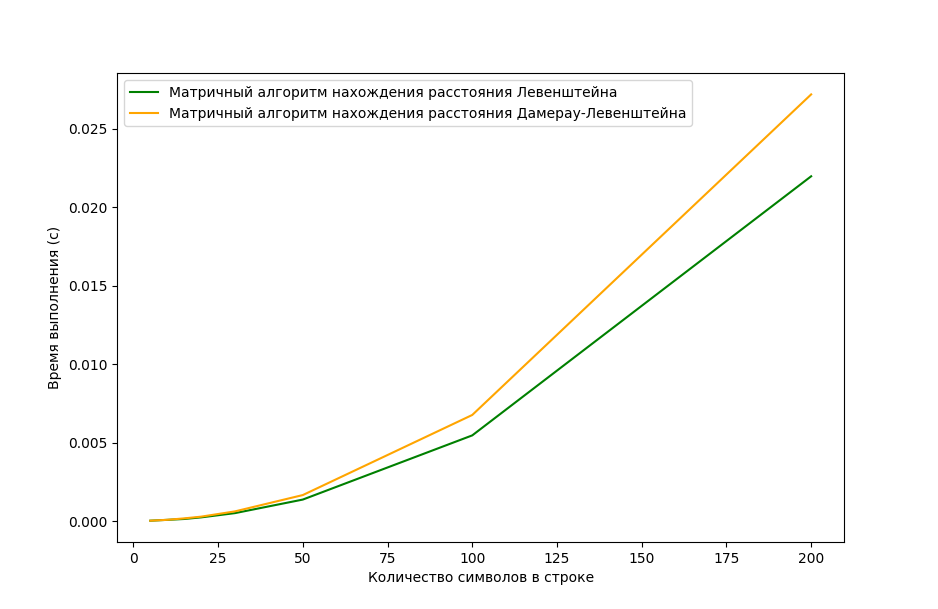
\includegraphics[scale=0.7]{time1.png}
	 \caption{Зависимость времени работы алгоритмов от длины строк. Часть1.}
	\end{center}
	\label{fig:plot}
\end{figure}

\begin{figure}[h]
	\begin{center}
	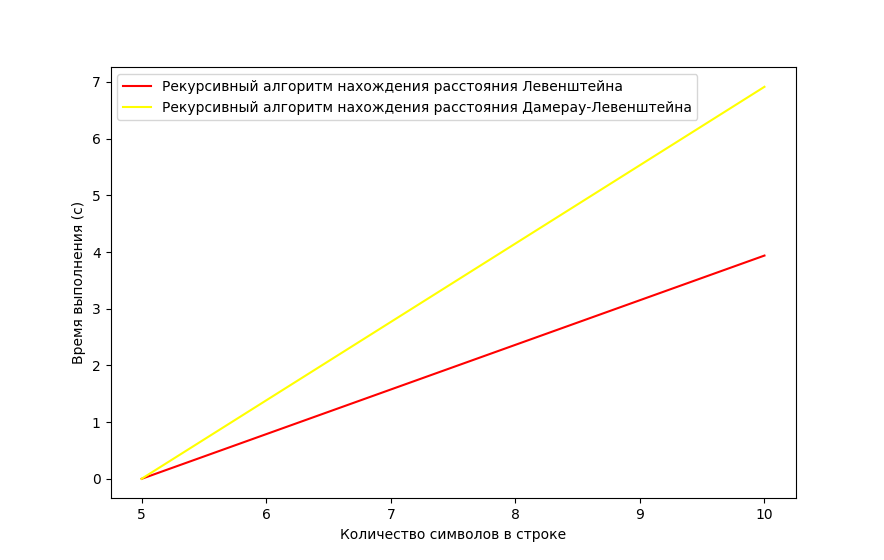
\includegraphics[scale=0.7]{time2.png}
	 \caption{Зависимость времени работы алгоритмов от длины строк. Часть2.}
	\end{center}
	\label{fig:plot}
\end{figure}

\subsection{Вывод}
	Наиболее эффективными по времени при маленькой длине слова являются рекурсивные реализации алгоритмов, но как только увеличивается длина слова, их эффективность резко снижается, что обусловлено большим количеством повторных рассчетов. Время работы алгоритма, использующего матрицу, намного меньше благодаря тому, что в нем требуется только (m + 1)*(n + 1) операций заполнения ячейки матрицы. Также установлено, что алгоритм Дамерау-Левенштейна работает немного дольше алгоритма Левенштейна, т.к. в нем добавлены дополнительные проверки, однако алгоритмы сравнимы по временной эффективности.

	

	\anonsection{Заключение}

	Был изучен метод динамического программирования на материале алгоритмов Левенштейна и Дамерау-Левенштейна.
	Также изучены алгоритмы Левенштейна и Дамерау-Левенштейна нахождения расстояния между строками, получены практические навыки раелизации указанных алгоритмов
	в матричной  и рекурсивных версиях. 
	\newline

	Экспериментально было подтверждено различие во временной эффективности рекурсивной и нерекурсивной реализаций выбранного алгоритма определения расстояния между строками при помощи разработаного программного обеспечения на материале замеров процессорного времени выполнения реализации на варьирующихся длинах строк. 
	\newline

	В результате исследований можно сделать вывод, что матричная реализация данных алгоритмов заметно выигрывает по времени при росте длины строк, следовательно более применима в реальных проектах.
	\newline
	
	При выполнение данной лабораторной работы была выполнена цель и достигнуты следующие задачи:

	\begin{itemize}
		\item были изучены алгоритмов Левенштейна и Дамерау-Левенштейна нахождения расстояния между строками;
		\item были применены методы динамического программирования для матричной реализации указанных алгоритмов;
		\item были получены практические навыки реализации указанных алгоритмов: двух алгоритмов в матричной версии и одного из алгоритмов в рекурсивной версии;
		\item были проведен сравнительный анализ линейной и рекурсивной реализаций выбранного алгоритма определения расстояния между строками по затрачиваемым ресурсам (времени и памяти);
		\item было экспериментально подтверждено различие во временнoй эффективности рекурсивной и нерекурсивной реализаций выбранного алгоритма определения расстояния между строками при помощи разработанного программного обеспечения на материале замеров процессорного времени выполнения реализации на варьирующихся длинах строк;
		\item были описаны и обоснованы полученные результаты в отчете о выполненной лабораторной работе, выполненного как расчётно-пояснительная записка к работе.
	\end{itemize}

	\anonsection{Список литературы}

	\begin{enumerate}

		\item В. И. Левенштейн. Двоичные коды с исправлением выпадений, вставок и замещений символов. Доклады Академий Наук СССР, 1965. 845-848.
		\item М. Лутц . Изучаем Python. O’REILLY, 2019. 731-732.
		\item Васильев. А. Н. Python на примерах. Практический курс по программированию. СПб.: Наука и Техника, 2016. 175-214.
		\item Л. Рамальо. Python. К вершинам мастерства. O’REILLY,, 2016. 44 - 68.
		\item Д. Хеллман. Стандартная библиотека Python 3. Компьютерное издательство “Диалектика'', 2019. 237-247.

	\end{enumerate}

\end{document}
